\section{Line Integrals}

%%%%%%%%%%%%%%%%%%%
%  Vector Fields  %
%%%%%%%%%%%%%%%%%%%

\subsection{Vector Fields}

\Definition{Vector Field}{
    A vector field on two or three dimensional space is a function $\vec{F}$ that assigns to each point $(x,y)$ or $(x,y,z)$ a two or three dimensional vector given by $\vec{F}(x,y)$ or $\vec{F}(x,y,z)$.
}

We can write vector fields in component form as follows. In two dimensions:
\[
    \vec{F}(x,y) = P(x,y)\,\vec{i} + Q(x,y)\,\vec{j}
\]
In three dimensions:
\[
    \vec{F}(x,y,z) = P(x,y,z)\,\vec{i} + Q(x,y,z)\,\vec{j} + R(x,y,z)\,\vec{k}
\]
where $P$, $Q$, and $R$ are scalar functions called the component functions of the vector field.

\Definition{Gradient Vector Fields}{
    If $f$ is a scalar function, then its gradient $\nabla f$ is a vector field. We call $\nabla f$ a \textbf{gradient vector field}. \\
    In two dimensions:
    \[
        \nabla f = \langle f_x, f_y \rangle = \pdv{f}{x}\,\vec{i} + \pdv{f}{y}\,\vec{j}
    \]
    In three dimensions:
    \[
        \nabla f = \langle f_x, f_y, f_z \rangle = \pdv{f}{x}\,\vec{i} + \pdv{f}{y}\,\vec{j} + \pdv{f}{z}\,\vec{k}
    \]
}

\begin{figure}[htpb]
    \centering
    \begin{subfigure}{0.4\textwidth}
        
\includegraphics[width=0.8\textwidth]{5.1.1.png}
        \caption{$\vec{F}(x,y) = -y\hat{i} + x\hat{j}$}
    \end{subfigure}
    \begin{subfigure}{0.4\textwidth}
        
\includegraphics[width=0.8\textwidth]{5.1.2.png}
        \caption{$\vec{F}(x,y,z) = 2x \hat{i} - 2y \hat{j} - 2x \hat{k}$}
    \end{subfigure}
    \caption{Examples of vector fields in (a) two dimensions and (b) three dimensions.}
    \label{fig:vector-field}
\end{figure}

\Definition{Conservative Vector Field}{
    A vector field $\vec{F}$ is called \textbf{conservative} if there exists a scalar function $f$ such that $\vec{F} = \nabla f$. The function $f$ is called a \textbf{potential function} for the vector field $\vec{F}$. \\
    In other words, a vector field is conservative if it can be expressed as the gradient of some scalar function.
}

For example, the vector field $\vec{F}=y \hat{i}+x \hat{j}$ is a conservative vector field with a potential function of $f(x,y)=xy$ because $\nabla f = \langle y,x \rangle$.

%%%%%%%%%%%%%%%%%%%%%%%%%%%%%%%%%
% Line Integrals wrt Arc Length %
%%%%%%%%%%%%%%%%%%%%%%%%%%%%%%%%%

\subsection{Line Integrals wrt Arc Length}

In this section we will look at line integrals with respect to arc length.

\Definition{Smooth Curve}{
    For a curve $C$ defined by the parametric equations \[ 
        x=x(t) \quad y=y(t) \quad a \leq t \leq b
    \] \[ 
        \text{or } \vec{r}(t) = x(t) \hat{i} + y(t) \hat{j} \quad a \leq t \leq b
    \]
    the curve is called \textbf{smooth} if $\vec{r'}(t)$ is continuous and $\vec{r'}(t) \neq 0$ for all $t$.
}

\Definition{Line Integral}{
    The \textbf{line integral} of $f(x,y)$ along a smooth curve $C$ is given by \[ 
        \int \limits_{C} f(x,y) \dd{s}
     \]
}

Here, $\dd{s}$ is used to denote a small segment of arc length along the curve $C$. For this reason, this is sometimes called the \textbf{line integral of $f$ with respect to arc length}. \\

Recall that $\dd{s} = \lVert \vec{r}'(t) \rVert \dd{t}$ where $\vec{r}(t) = \langle x(t), y(t) \rangle$ is the position vector for the curve. Therefore: \[
    \dd{s} = \lVert \vec{r'}(t) \rVert \dd{t} = \sqrt{\left(\dv{x}{t}\right)^2 + \left(\dv{y}{t}\right)^2} \dd{t}
\]

\Note[Line Integral with Respect to Arc Length]{
    The line integral of $f$ along $C$ with respect to arc length is: \[
        \int \limits_{C} f(x,y) \dd{s} = \int_a^b f(x(t), y(t)) \sqrt{\left(\dv{x}{t}\right)^2 + \left(\dv{y}{t}\right)^2} \dd{t}
    \]

    For three-dimensional curves given by $\vec{r}(t) = \langle x(t), y(t), z(t) \rangle$ where $a \le t \le b$: \[
        \int \limits_{C} f(x,y,z) \dd{s} = \int_a^b f(x(t), y(t), z(t)) \sqrt{\left(\dv{x}{t}\right)^2 + \left(\dv{y}{t}\right)^2 + \left(\dv{z}{t}\right)^2} \dd{t}
    \]
}

\Example{Evaluate $\int \limits_{C} xyz \dd{s}$ where $C$ is the curve given by $\langle \cos(t), \sin(t), 3t \rangle$, $0 \leq t \leq 4\pi$.}{
    First, we compute $\dd{s}$:
    \begin{align*}
        \vec{r}'(t) &= \langle -\sin(t), \cos(t), 3 \rangle \\
        \lVert \vec{r}'(t) \rVert &= \sqrt{(-\sin(t))^2 + (\cos(t))^2 + (3)^2} = \sqrt{1 + 9} = \sqrt{10} \\
        \dd{s} &= \sqrt{10} \dd{t}
    \end{align*}
    Next, we evaluate the function along the curve: \[
        f(x(t), y(t), z(t)) = (\cos(t))(\sin(t))(3t) = 3t\cos(t)\sin(t)
    \]
    Now we can set up the line integral:
    \begin{align*}
        \int \limits_{C} xyz \dd{s} &= \int_0^{4\pi} 3t\cos(t)\sin(t) \sqrt{10} \dd{t} \\
        &= 3\sqrt{10} \int_0^{4\pi} t\cos(t)\sin(t) \dd{t} \\
        &= \frac{3\sqrt{10}}{2} \int_0^{4\pi} t\sin(2t) \dd{t}
    \end{align*}
    To evaluate $\int_0^{4\pi} t\sin(2t) \dd{t}$, we use integration by parts. Let $u = t$ and $\dd{v} = \sin(2t) \dd{t}$. Then $\dd{u} = \dd{t}$ and $v = -\frac{1}{2}\cos(2t)$. Thus:
    \begin{align*}
        \int \limits_{C} xyz \dd{s} &= \frac{3 \sqrt{10}}{2} \left[ -\frac{t}{2}\cos(2t) + \frac{1}{2} \int \limits_0^{4\pi} \cos(2t) \dd{t} \right]_0^{4\pi} \\
                                    &= \frac{3 \sqrt{10}}{2} \left[ -\frac{t}{2}\cos(2t) + \frac{1}{4}\sin(2t) \right]_0^{4\pi} \\
                                    &= \frac{3 \sqrt{10}}{2} \left( -\frac{4\pi}{2}\cos(8\pi) + \frac{1}{4}\sin(8\pi) - 0 \right) \\
                                    &= \frac{3 \sqrt{10}}{2} \left( -2\pi(1) + 0 \right) \\
                                    &= -3\pi \sqrt{10}
    \end{align*}
}

\Definition{Piecewise Smooth Curves}{
    If a curve $C$ is not smooth, but can be broken into a finite number of smooth pieces $C_1, C_2, \ldots, C_n$, then $C$ is called \textbf{piecewise smooth}, and the line integral along $C$ is defined as: \[
        \int \limits_{C} f \dd{s} = \sum_{i=1}^n \int \limits_{C_i} f \dd{s}
    \]
}

\Note[Direction Independence]{
    For line integrals with respect to arc length, changing the direction of the curve does \textbf{not} change the value of the integral. That is: \[
        \int \limits_{C} f \dd{s} = \int \limits_{-C} f \dd{s}
    \]
    where $-C$ denotes the curve $C$ traversed in the opposite direction.
}

%%%%%%%%%%%%%%%%%%%%%%%%%%%%
% Line Integrals wrt x,y,z %
%%%%%%%%%%%%%%%%%%%%%%%%%%%%

\subsection{Line Integrals wrt $x$, $y$, $z$}

\Note[ Line Integral with Respect to $x$ and $y$ ]{
    For a two-dimensional curve $C$ with parameterization $x = x(t)$, $y = y(t)$, $a \le t \le b$: \\
    The \textbf{line integral of $f$ with respect to $x$} is: \[
        \int \limits_{C} f(x,y) \dd{x} = \int_a^b f(x(t), y(t)) \dv{x}{t} \dd{t}
    \]
    The \textbf{line integral of $f$ with respect to $y$} is: \[
        \int \limits_{C} f(x,y) \dd{y} = \int_a^b f(x(t), y(t)) \dv{y}{t} \dd{t}
    \]
}

\Note{
    These integrals often appear together, so we use the following shorthand notation: \[
        \int \limits_{C} P \dd{x} + Q \dd{y} = \int \limits_{C} P(x,y) \dd{x} + \int \limits_{C} Q(x,y) \dd{y}
    \]
}

\Example{Evaluate $\int \limits_{C} \sin(\pi y) \dd{y} + yx^2 \dd{x}$ where $C$ is the line segment from $(0,2)$ to $(1,4)$.}{
    First, parameterize the curve: \[
        \vec{r}(t) = (1-t)\langle 0,2 \rangle + t\langle 1,4 \rangle = \langle t, 2+2t \rangle, \quad 0 \le t \le 1
    \]
    
    So $x(t) = t$, $y(t) = 2+2t$, and: \[
        \dv{x}{t} = 1 \quad \dv{y}{t} = 2
    \]
    
    Now evaluate the line integral:
    \begin{align*}
        \int \limits_{C} \sin(\pi y) \dd{y} + yx^2 \dd{x} &= \int_0^1 \sin(\pi(2+2t))(2) \dd{t} + \int_0^1 (2+2t)(t)^2(1) \dd{t} \\
        &= \int_0^1 2\sin(2\pi + 2\pi t) \dd{t} + \int_0^1 (2t^2 + 2t^3) \dd{t} \\
        &= \left[-\frac{1}{\pi}\cos(2\pi + 2\pi t)\right]_0^1 + \left[\frac{2t^3}{3} + \frac{t^4}{2}\right]_0^1 \\
        &= -\frac{1}{\pi}(\cos(4\pi) - \cos(2\pi)) + \frac{2}{3} + \frac{1}{2} \\
        &= -\frac{1}{\pi}(1 - 1) + \frac{4 + 3}{6} \\
        &= 0 + \frac{7}{6} = \frac{7}{6}
    \end{align*}
}

\Note{
    For three-dimensional curves $C$ with parameterization $x = x(t)$, $y = y(t)$, $z = z(t)$, $a \le t \le b$:
    \begin{align*}
        \int \limits_{C} f(x,y,z) \dd{x} &= \int_a^b f(x(t), y(t), z(t)) \dv{x}{t} \dd{t} \\
        \int \limits_{C} f(x,y,z) \dd{y} &= \int_a^b f(x(t), y(t), z(t)) \dv{y}{t} \dd{t} \\
        \int \limits_{C} f(x,y,z) \dd{z} &= \int_a^b f(x(t), y(t), z(t)) \dv{z}{t} \dd{t}
    \end{align*}
}

\Note{
    The shorthand notation for the combined form is:
    \[
        \int \limits_{C} P \dd{x} + Q \dd{y} + R \dd{z} = \int \limits_{C} P(x,y,z) \dd{x} + \int \limits_{C} Q(x,y,z) \dd{y} + \int \limits_{C} R(x,y,z) \dd{z}
    \]
}

\Example{Evaluate $\int \limits_{C} y \dd{x} + x \dd{y} + z \dd{z}$ where $C$ is given by $x = \cos t$, $y = \sin t$, $z = t^2$ for $0 \le t \le 2\pi$.}{
    We have $x(t) = \cos t$, $y(t) = \sin t$, and $z(t) = t^2$.
    
    Compute the derivatives: \[
        \dv{x}{t} = -\sin t \quad \dv{y}{t} = \cos t \quad \dv{z}{t} = 2t
    \]
    
    Evaluate the line integral:
    \begin{align*}
        \int \limits_{C} y \dd{x} + x \dd{y} + z \dd{z} &= \int_0^{2\pi} \sin t(-\sin t) \dd{t} + \int_0^{2\pi} \cos t(\cos t) \dd{t} + \int_0^{2\pi} t^2(2t) \dd{t} \\
        &= \int_0^{2\pi} (-\sin^2 t + \cos^2 t + 2t^3) \dd{t} \\
        &= \int_0^{2\pi} \cos(2t) \dd{t} + \int_0^{2\pi} 2t^3 \dd{t} \\
        &= \frac{1}{2}\sin(2t)\Biggr|_{0}^{2\pi} + \frac{t^4}{2}\Biggr|_{0}^{2\pi} \\
        &= 0 + \frac{(2\pi)^4}{2} = 8\pi^4
    \end{align*}
}

\Note[Direction Dependence]{
    For line integrals with respect to $x$, $y$, and/or $z$, changing the direction of the curve \textbf{does} change the value of the integral by a factor of $-1$. That is:
    \[
        \int \limits_{-C} f(x,y) \dd{x} = -\int \limits_{C} f(x,y) \dd{x} \quad \text{and} \quad \int \limits_{-C} f(x,y) \dd{y} = -\int \limits_{C} f(x,y) \dd{y}
    \]
    
    For the combined form:
    \[
        \int \limits_{-C} P \dd{x} + Q \dd{y} = -\int \limits_{C} P \dd{x} + Q \dd{y}
    \]
}

%%%%%%%%%%%%%%%%%%%%%%%%%%%%%%%%%%%
% Line Integrals of Vector Fields %
%%%%%%%%%%%%%%%%%%%%%%%%%%%%%%%%%%%

\subsection{Line Integrals of Vector Fields}

Let a three-dimensional vector field be \[ 
    \vec{F}(x,y,z) = P(x,y,z)\,\vec{i} + Q(x,y,z)\,\vec{j} + R(x,y,z)\,\vec{k}
\]
and let $C$ a three-dimensional smooth curve be given by: \[
    \vec{r}(t) = x(t)\,\vec{i} + y(t)\,\vec{j} + z(t)\,\vec{k}, \quad a \le t \le b
\]

\Definition{Line Integral of a Vector Field}{
    The \textbf{line integral of $\vec{F}$ along $C$} is:
    \[
        \int \limits_{C} \vec{F} \cdot \dd{\vec{r}} = \int_a^b \vec{F}(\vec{r}(t)) \cdot \vec{r}'(t) \dd{t}
    \]
}

Note: \[ 
    \vec{F}(\vec{r}(t)) = \vec{F}(x(t), y(t), z(t))
\]

\Note[Alternative Notation]{
    We can also write line integrals of vector fields using the unit tangent vector $\vec{T}$:
    \[
        \int \limits_{C} \vec{F} \cdot \dd{\vec{r}} = \int \limits_{C} \vec{F} \cdot \vec{T} \dd{s}
    \]
    where $\vec{T}(t) = \dfrac{\vec{r}'(t)}{\|\vec{r}'(t)\|}$ is the unit tangent vector.
}

\Note[Relationship to Line Integrals with Respect to Coordinates]{
    Line integrals of vector fields are related to line integrals with respect to $x$, $y$, and $z$:
    \[
        \int \limits_{C} \vec{F} \cdot \dd{\vec{r}} = \int \limits_{C} P \dd{x} + Q \dd{y} + R \dd{z}
    \]
    
    To see this, note that:
    \begin{align*}
        \int \limits_{C} \vec{F} \cdot \dd{\vec{r}} &= \int_a^b (P\,\vec{i} + Q\,\vec{j} + R\,\vec{k}) \cdot (x'\,\vec{i} + y'\,\vec{j} + z'\,\vec{k}) \dd{t} \\
        &= \int_a^b (Px' + Qy' + Rz') \dd{t} \\
        &= \int_a^b Px' \dd{t} + \int_a^b Qy' \dd{t} + \int_a^b Rz' \dd{t} \\
        &= \int \limits_{C} P \dd{x} + \int \limits_{C} Q \dd{y} + \int \limits_{C} R \dd{z}
    \end{align*}
}

\Example{Evaluate $\int \limits_{C} \vec{F} \cdot \dd{\vec{r}}$ where $\vec{F}(x,y,z) = 8x^2yz\,\vec{i} + 5z\,\vec{j} - 4xy\,\vec{k}$ and $C$ is given by $\vec{r}(t) = t\,\vec{i} + t^2\,\vec{j} + t^3\,\vec{k}$ for $0 \le t \le 1$.}{
    First, evaluate the vector field along the curve:
    \[
        \vec{F}(\vec{r}(t)) = 8t^2(t^2)(t^3)\,\vec{i} + 5t^3\,\vec{j} - 4t(t^2)\,\vec{k} = 8t^7\,\vec{i} + 5t^3\,\vec{j} - 4t^3\,\vec{k}
    \]
    
    Next, compute the derivative of the parameterization:
    \[
        \vec{r}'(t) = \vec{i} + 2t\,\vec{j} + 3t^2\,\vec{k}
    \]
    
    Now compute the dot product:
    \begin{align*}
        \vec{F}(\vec{r}(t)) \cdot \vec{r}'(t) &= (8t^7)(1) + (5t^3)(2t) + (-4t^3)(3t^2) \\
        &= 8t^7 + 10t^4 - 12t^5
    \end{align*}
    
    Finally, evaluate the integral:
    \begin{align*}
        \int \limits_{C} \vec{F} \cdot \dd{\vec{r}} &= \int_0^1 (8t^7 + 10t^4 - 12t^5) \dd{t} \\
        &= \left[t^8 + 2t^5 - 2t^6\right]_0^1 \\
        &= 1 + 2 - 2 = 1
    \end{align*}
}

\Example{Evaluate $\int \limits_{C} \vec{F} \cdot \dd{\vec{r}}$ where $\vec{F}(x,y,z) = xz\,\vec{i} - yz\,\vec{k}$ and $C$ is the line segment from $(-1,2,0)$ to $(3,0,1)$.}{
    First, parameterize the line segment:
    \begin{align*}
        \vec{r}(t) &= (1-t)\langle -1,2,0 \rangle + t\langle 3,0,1 \rangle \\
        &= \langle 4t-1, 2-2t, t \rangle, \quad 0 \le t \le 1
    \end{align*}
    
    Evaluate the vector field along the curve:
    \begin{align*}
        \vec{F}(\vec{r}(t)) &= (4t-1)(t)\,\vec{i} - (2-2t)(t)\,\vec{k} \\
        &= (4t^2-t)\,\vec{i} - (2t-2t^2)\,\vec{k}
    \end{align*}
    
    Compute the derivative:
    \[
        \vec{r}'(t) = \langle 4, -2, 1 \rangle
    \]
    
    Compute the dot product:
    \begin{align*}
        \vec{F}(\vec{r}(t)) \cdot \vec{r}'(t) &= (4t^2-t)(4) + 0(-2) + (-2t+2t^2)(1) \\
        &= 16t^2 - 4t - 2t + 2t^2 \\
        &= 18t^2 - 6t
    \end{align*}
    
    Evaluate the integral:
    \begin{align*}
        \int \limits_{C} \vec{F} \cdot \dd{\vec{r}} &= \int_0^1 (18t^2 - 6t) \dd{t} \\
        &= \left[6t^3 - 3t^2\right]_0^1 \\
        &= 6 - 3 = 3
    \end{align*}
}

\Note[Work Interpretation]{
    In physics, if $\vec{F}$ represents a force field and $C$ is the path taken by an object, then $\int \limits_{C} \vec{F} \cdot \dd{\vec{r}}$ represents the \textbf{work} done by the force field in moving the object along the path $C$.
}

\Note[Direction Dependence for Vector Fields]{
    As with line integrals with respect to coordinates, reversing the direction of the curve changes the sign of the integral:
    \[
        \int \limits_{-C} \vec{F} \cdot \dd{\vec{r}} = -\int \limits_{C} \vec{F} \cdot \dd{\vec{r}}
    \]
}

\Note{
    We can write vector fields in component form as follows: \[
        \vec{F}(x,y,z) = P(x,y,z)\,\vec{i} + Q(x,y,z)\,\vec{j} + R(x,y,z)\,\vec{k}
    \]
    where $P$, $Q$, and $R$ are scalar functions called the component functions of the vector field.
}

\Note[Gradient Vector Fields]{
    If $f$ is a scalar function, then its gradient $\nabla f$ is a vector field. We call $\nabla f$ a \textbf{gradient vector field}. In two dimensions:
    \[
        \nabla f = \pdv{f}{x}\,\vec{i} + \pdv{f}{y}\,\vec{j}
    \]
    In three dimensions:
    \[
        \nabla f = \pdv{f}{x}\,\vec{i} + \pdv{f}{y}\,\vec{j} + \pdv{f}{z}\,\vec{k}
    \]
}


%%%%%%%%%%%%%%%%%%%%%%%%%%%%%%%%%%%%%%%%%%%%
%  Fundamental Theorem for Line Integrals  %
%%%%%%%%%%%%%%%%%%%%%%%%%%%%%%%%%%%%%%%%%%%%

\subsection{Fundamental Theorem for Line Integrals}

\Theorem{Fundamental Theorem for Line Integrals}{
    Let $C$ be a smooth curve given by $\vec{r}(t), a \leq t \leq b$. Also, let $f$ be a differentiable scalar function whose gradient vector field $\nabla f$ is continuous on $C$. Then:
    \[ 
        \int \limits_{C} \nabla f \cdot \dd{\vec{r}} = f(\vec{r}(b)) - f(\vec{r}(a))
    \]
}

\underline{\textbf{Proof:}} \\
By definition of the line integral of a vector field, we have:
\begin{align*}
    \int \limits_{C} \nabla f \cdot \dd{\vec{r}} &= \int_a^b \nabla f(\vec{r}(t)) \cdot \vec{r}'(t) \dd{t} \\
                                                 &= \int_a^b \left( \pdv{f}{x} \dv{x}{t} + \pdv{f}{y} \dv{y}{t} + \pdv{f}{z} \dv{z}{t} \right) \dd{t} \\
                                                 &= \int_a^b \dv{}{t} [f(\vec{r}(t))] \dd{t} \\
                                                 &= f(\vec{r}(b)) - f(\vec{r}(a)) \qed
\end{align*}

\Example{Evaluate $\displaystyle \int \limits_{C} \nabla f \cdot \dd{\vec{r}}$ where $f(x,y,z) = \cos(\pi x) + \sin(\pi y) - xyz$ and C is any path that starts at $\left( 1, \frac{1}{2}, 2 \right)$ and ends at $(2,1,-1)$.}{
    By the Fundamental Theorem for Line Integrals, we have:
    \begin{align*}
        \int \limits_{C} \nabla f \cdot \dd{\vec{r}} &= f(2,1,-1) - f\left( 1, \frac{1}{2}, 2 \right) \\
        &= \left[ \cos(2\pi) + \sin(\pi) - (2)(1)(-1) \right] - \left[ \cos(\pi) + \sin\left( \frac{\pi}{2} \right) - (1)\left( \frac{1}{2} \right)(2) \right] \\
        &= [1 + 0 + 2] - [-1 + 1 - 1] \\
        &= 3 - (-1) = 4
    \end{align*}
}

\Definition{}{
    \begin{enumerate}[leftmargin=150pt]
        \item[Conservative Vector Field:] A vector field $\vec{F}$ is called \textbf{conservative} if there exists a scalar function $f$ such that $\vec{F} = \nabla f$. The function $f$ is called a \textbf{potential function} for the vector field $\vec{F}$.
        \item[Path Independence:] A line integral $\displaystyle \int \limits_{C} \vec{F} \cdot \dd{\vec{r}}$ is called \textbf{path independent} if its value depends only on the endpoints of the curve $C$ and not on the specific path taken between those points.
        \item[Closed Curve:] A curve $C$ is called \textbf{closed} if its initial point and terminal point are the same.
        \item[Simple Curve:] A curve $C$ in $\R^2$ or $\R^3$ is called \textbf{simple} if it does not intersect itself, except possibly at the endpoints if it is closed.
        \item[Open Region:] A region $D$ in $\R^2$ or $\R^3$ is called \textbf{open} if for every point in $D$, there exists a small neighborhood around that point which is entirely contained within $D$. Simply put, an open region does not include its boundary points.
        \item[Connected Region:] A region $D$ in $\R^2$ or $\R^3$ is called \textbf{connected} if any two points in $D$ can be joined by a curve that lies entirely within $D$.
        \item[Simply Connected Region:] A region $D$ in $\R^2$ or $\R^3$ is called \textbf{simply connected} if any closed curve in $D$ can be continuously contracted to a point without leaving $D$. Simply put, a simply connected region has no holes.
    \end{enumerate}
}

\Note{
    \begin{enumerate}
        \item $\displaystyle \int \limits_{C} \nabla f \cdot \dd{\vec{r}}$ is independent of path.
        \item If $\vec{F}$ is a conservative vector field, then $\displaystyle \int \limits_{C} \vec{F} \cdot \dd{\vec{r}}$ is independent of path.
        \item If $\vec{F}$ is a continuous vector field on an open connected region $D$ and if $\displaystyle \int \limits_{C} \vec{F} \cdot \dd{\vec{r}}$ is independent of path (for any path in $D$), then $\vec{F}$ is a conservative vector field on $D$.
        \item If $\displaystyle \int \limits_{C} \vec{F} \cdot \dd{\vec{r}}$ is independent of path, then $\displaystyle \int \limits_{C} \vec{F} \cdot \dd{\vec{r}} = 0$ for every closed path $C$.
        \item If $\int \limits_{C} \vec{F} \cdot \dd{\vec{r}} = 0$ for every closed path $C$, then $\displaystyle \int \limits_{C} \vec{F} \cdot \dd{\vec{r}}$ is independent of path.
    \end{enumerate}
}


%%%%%%%%%%%%%%%%%%%%%%%%%%%%%%%%
%  Conservative Vector Fields  %
%%%%%%%%%%%%%%%%%%%%%%%%%%%%%%%%

\subsection{Conservative Vector Fields}

\Theorem{Characterization of Conservative Vector Fields in $\R^2$}{
    Let $\vec{F}(x,y) = P(x,y)\,\vec{i} + Q(x,y)\,\vec{j}$ be a vector field defined on an \textbf{open} and \textbf{simply connected} region $D$ of $\R^2$, where $P$ and $Q$ have continuous first partial derivatives in $D$. Then $\vec{F}$ is a conservative vector field if and only if: \[
        \pdv{P}{y} = \pdv{Q}{x}
    \]
}

\Note[Finding Potential Functions in $\R^2$]{
    Now that we have a way to determine if a vector field is conservative, we can find its potential function. We can say that \[ 
        \nabla f = \pdv{f}{x} \hat{i} + \pdv{f}{y} \hat{j} = P \hat{i} + Q \hat{j} = \vec{F}
    \]
    Equating components, we have: \[
        \pdv{f}{x} = P(x,y) \quad \text{and} \quad \pdv{f}{y} = Q(x,y)
    \]
    Then, to find $f$, we can integrate $P$ with respect to $x$ and $Q$ with respect to $y$. \[ 
        f(x,y) = \int P(x,y) \dd{x} \quad \text{and} \quad f(x,y) = \int Q(x,y) \dd{y}
    \]
}

\Note[Finding Potential Functions in $\R^3$]{
    Similarly, for a vector field in $\R^3$: \[
        \nabla f = \pdv{f}{x} \hat{i} + \pdv{f}{y} \hat{j} + \pdv{f}{z} \hat{k} = P \hat{i} + Q \hat{j} + R \hat{k} = \vec{F}
    \]
    Equating components, we have: \[
        \pdv{f}{x} = P(x,y,z) \quad \pdv{f}{y} = Q(x,y,z) \quad \text{and} \quad \pdv{f}{z} = R(x,y,z)
    \]
    Then, to find $f$, we can integrate $P$ with respect to $x$, $Q$ with respect to $y$, and $R$ with respect to $z$. \[
        f(x,y,z) = \int P(x,y,z) \dd{x} \quad f(x,y,z) = \int Q(x,y,z) \dd{y} \quad f(x,y,z) = \int R(x,y,z) \dd{z}
    \]
}


%%%%%%%%%%%%%%%%%%%%%
%  Green's Theorem  %
%%%%%%%%%%%%%%%%%%%%%

\subsection{Green's Theorem}

Green's Theorem establishes a relationship between certain line integrals on closed paths and double integrals over the region enclosed by the path.

\Definition{Positively Oriented Curve}{
    A simple closed curve $C$ is \textbf{positively oriented} if it is traced out in a counter-clockwise direction. Equivalently, as we traverse the path following the positive orientation, the region $D$ enclosed by $C$ is always on the left.
}

\Theorem{Green's Theorem}{
    Let $C$ be a positively oriented, piecewise smooth, simple closed curve, and let $D$ be the region bounded by $C$. If $P$ and $Q$ have continuous first order partial derivatives on an open region that contains $D$, then:
    \[
        \oint \limits_{C} P \dd{x} + Q \dd{y} = \iint \limits_{D} \left( \pdv{Q}{x} - \pdv{P}{y} \right) \dd{A}
    \]
}

\Note[Notation for Closed Curves]{
    When working with a line integral in which the path satisfies the conditions of Green's Theorem, we often denote the line integral as:
    \[
        \oint \limits_{C} P \dd{x} + Q \dd{y}
    \]
    The circle on the integral sign indicates that $C$ is a closed curve. Sometimes the curve $C$ is viewed as the boundary of region $D$ and is denoted as $\partial D$.
}

\Example{Use Green's Theorem to evaluate $\displaystyle \oint \limits_{C} xy \dd{x} + x^2y^3 \dd{y}$ where $C$ is the triangle with vertices $(0,0)$, $(1,0)$, $(1,2)$ with positive orientation.}{
    \begin{minipage}[t]{0.55\textwidth}
        The region $D$ can be described by: \[
            0 \le x \le 1, \quad 0 \le y \le 2x
        \]
        Next, identify $P$ and $Q$: \[
            P(x,y) = xy \qquad Q(x,y) = x^2y^3
        \]
        Compute the partial derivatives: \[
            \pdv{Q}{x} = 2xy^3 \qquad \pdv{P}{y} = x
        \]
    \end{minipage}\hfill
    \begin{minipage}[t]{0.4\textwidth}
        \centering\vspace{0pt}
        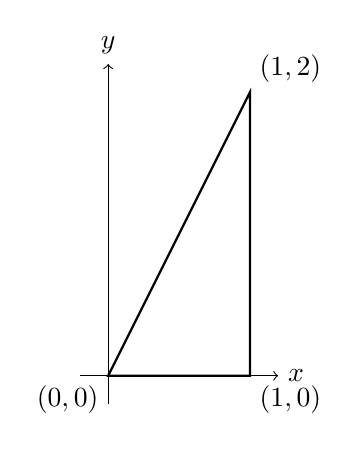
\begin{tikzpicture}[scale=1.8]
            % Axes
            \draw[->] (-0.2,0) -- (1.2,0) node[right] {$x$};
            \draw[->] (0,-0.2) -- (0,2.2) node[above] {$y$};
            % Triangle
            \draw[thick] (0,0) -- (1,0) -- (1,2) -- cycle;
            % Labels
            \node at (0,0) [below left] {$(0,0)$};
            \node at (1,0) [below right] {$(1,0)$};
            \node at (1,2) [above right] {$(1,2)$};
        \end{tikzpicture}
    \end{minipage}

    Apply Green's Theorem:
    \begin{align*}
        \oint \limits_{C} xy \dd{x} + x^2y^3 \dd{y} &= \iint \limits_{D} (2xy^3 - x) \dd{A} \\
        &= \int_0^1 \int_0^{2x} (2xy^3 - x) \dd{y} \dd{x} \\
        &= \int_0^1 \left[ \frac{1}{2}xy^4 - xy \right]_0^{2x} \dd{x} \\
        &= \int_0^1 \left( \frac{1}{2}x(2x)^4 - x(2x) \right) \dd{x} \\
        &= \int_0^1 (8x^5 - 2x^2) \dd{x} \\
        &= \left[ \frac{4x^6}{3} - \frac{2x^3}{3} \right]_0^1 \\
        &= \frac{4}{3} - \frac{2}{3} = \frac{2}{3}
    \end{align*}
}

\Example{Evaluate $\displaystyle \oint \limits_{C} y^3 \dd{x} - x^3 \dd{y}$ where $C$ is the positively oriented circle of radius 2 centered at the origin.}{
    Identify $P$ and $Q$:
    \[
        P(x,y) = y^3 \qquad Q(x,y) = -x^3
    \]
    
    Be careful with the minus sign on $Q$!
    
    Compute the partial derivatives:
    \[
        \pdv{Q}{x} = -3x^2 \qquad \pdv{P}{y} = 3y^2
    \]
    
    Apply Green's Theorem where $D$ is the disk of radius 2:
    \begin{align*}
        \oint \limits_{C} y^3 \dd{x} - x^3 \dd{y} &= \iint \limits_{D} (-3x^2 - 3y^2) \dd{A} \\
        &= -3 \iint \limits_{D} (x^2 + y^2) \dd{A}
    \end{align*}
    
    Since $D$ is a disk, use polar coordinates where $x^2 + y^2 = r^2$:
    \begin{align*}
        \oint \limits_{C} y^3 \dd{x} - x^3 \dd{y} &= -3 \int_0^{2\pi} \int_0^2 r^2 \cdot r \dd{r} \dd{\theta} \\
        &= -3 \int_0^{2\pi} \int_0^2 r^3 \dd{r} \dd{\theta} \\
        &= -3 \int_0^{2\pi} \left[ \frac{r^4}{4} \right]_0^2 \dd{\theta} \\
        &= -3 \int_0^{2\pi} 4 \dd{\theta} = -12 \theta \bigr|_{0}^{2\pi} = -24\pi
    \end{align*}
}

So far, the region $D$ was assumed to have no holes. However, many regions do have holes in them, and Green's Theorem can be extended to regions with holes.

Consider a region $D$ that looks like a ring (annulus) as shown in Figure~\ref{fig:greens-theorem-holes-a}. Let $C_1$ be the outer boundary and $C_2$ be the inner boundary (the hole). For Green's Theorem to work, we need both boundaries to be positively oriented relative to $D$.

\begin{figure}[htpb]
    \centering
    \begin{subfigure}{0.4\textwidth}
        \centering
        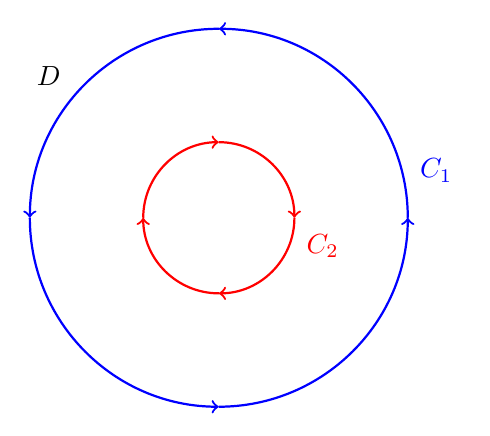
\begin{tikzpicture}[scale=1.2]
            % Outer boundary
            \draw[thick, blue, ->] (2,0) arc (0:90:2) node[midway, right] {};
            \draw[thick, blue, ->] (0,2) arc (90:180:2) node[midway, above] {};
            \draw[thick, blue, ->] (-2,0) arc (180:270:2) node[midway, left] {};
            \draw[thick, blue, ->] (0,-2) arc (270:360:2) node[midway, below] {};
            \node[blue] at (2.3,0.5) {$C_1$};
            % Inner boundary (clockwise)
            \draw[thick, red, ->] (0.8,0) arc (0:-90:0.8) node[midway, right] {};
            \draw[thick, red, ->] (0,-0.8) arc (-90:-180:0.8) node[midway, below] {};
            \draw[thick, red, ->] (-0.8,0) arc (180:90:0.8) node[midway, left] {};
            \draw[thick, red, ->] (0,0.8) arc (90:0:0.8) node[midway, above] {};
            \node[red] at (1.1,-0.3) {$C_2$};
            % Region label
            \node at (-1.8,1.5) {$D$};
        \end{tikzpicture}
        \caption{}
        \label{fig:greens-theorem-holes-a}
    \end{subfigure}
    \begin{subfigure}{0.4\textwidth}
        \centering
        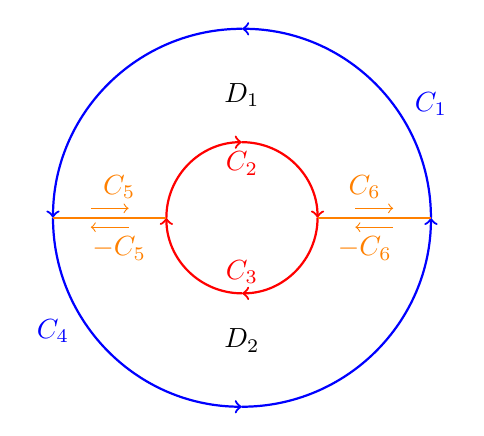
\begin{tikzpicture}[scale=1.2]
            % Outer boundary
            \draw[thick, blue, ->] (2,0) arc (0:90:2) node[midway, right] {};
            \draw[thick, blue, ->] (0,2) arc (90:180:2) node[midway, above] {};
            \draw[thick, blue, ->] (-2,0) arc (180:270:2) node[midway, left] {};
            \draw[thick, blue, ->] (0,-2) arc (270:360:2) node[midway, below] {};
            \node[blue] at (2.0,1.2) {$C_1$};
            \node[blue] at (-2.0,-1.2) {$C_4$};
            % Inner boundary (clockwise)
            \draw[thick, red, ->] (0.8,0) arc (0:-90:0.8) node[midway, right] {};
            \draw[thick, red, ->] (0,-0.8) arc (-90:-180:0.8) node[midway, below] {};
            \draw[thick, red, ->] (-0.8,0) arc (180:90:0.8) node[midway, left] {};
            \draw[thick, red, ->] (0,0.8) arc (90:0:0.8) node[midway, above] {};
            \node[red, below] at (0,0.8) {$C_2$};
            \node[red, above] at (0,-0.8) {$C_3$};
            % Region label
            \node at (0,1.3) {$D_1$};
            \node at (0,-1.3) {$D_2$};
            % Cut lines
            \draw[thick, orange] (0.8,0) -- (2,0);
            \draw[thick, orange] (-0.8,0) -- (-2,0);
            \node[orange, above] at (1.3,0.1) {$C_6$};
            \draw[orange, ->] (1.2,0.1) -- (1.6,0.1);
            \node[orange, below] at (1.3,-0.1) {$-C_6$};
            \draw[orange, ->] (1.6,-0.1) -- (1.2,-0.1);
            \node[orange, above] at (-1.3,0.1) {$C_5$};
            \draw[orange, ->] (-1.6,0.1) -- (-1.2,0.1);
            \node[orange, below] at (-1.3,-0.1) {$-C_5$};
            \draw[orange, ->] (-1.2,-0.1) -- (-1.6,-0.1);
        \end{tikzpicture}
        \caption{}
        \label{fig:greens-theorem-holes-b}
    \end{subfigure}
    \caption{(a) Region $D$ with outer boundary $C_1$ and inner boundary $C_2$. (b) Region $D$ cut into two sub-regions $D_1$ and $D_2$ along cut lines $C_5$ and $C_6$.}
    \label{fig:greens-theorem-holes}
\end{figure}

Now, since the region $D$ has a hole in it, we can't directly apply Green's Theorem. However, we can cut the disk in half and rename all the various portions of the curve as shown in Figure~\ref{fig:greens-theorem-holes-b}. Thus we have two regions $D_1$, which is bounded by $C_1 \cup C_2 \cup C_5 \cup C_6$ and $D_2$, which is bounded by $C_1 \cup C_2 \cup (-C_5) \cup (-C_6)$.

Now we can apply Green's Theorem to each of these two regions since they have no holes.

\begin{align*}
    \iint \limits_{D} (Q_x-P_y) \dd{A} &= \iint \limits_{D_1} (Q_x-P_y) \dd{A} + \iint \limits_{D_2} (Q_x-P_y) \dd{A} \\
                                       &= \oint \limits_{C_1 \cup C_2 \cup C_5 \cup C_6} P \dd{x} + Q \dd{y} + \oint \limits_{C_1 \cup C_2 \cup (-C_5) \cup (-C_6)} P \dd{x} + Q \dd{y}
\end{align*}

Now we can break up the line integrals. Also note that the integrals over $C_5$ and $-C_5$ cancel out, as do the integrals over $C_6$ and $-C_6$:
\begin{align*}
    \iint \limits_{D} (Q_x-P_y) \dd{A} &= \oint \limits_{C_1} P \dd{x} + Q \dd{y} + \oint \limits_{C_2} P \dd{x} + Q \dd{y} + \oint \limits_{C_3} P \dd{x} + Q \dd{y} + \oint \limits_{C_4} P \dd{x} + Q \dd{y} \\
                                       &= \oint \limits_{C_1 \cup C_2 \cup C_3 \cup C_4} P \dd{x}+ Q \dd{y} \\
                                       &= \oint \limits_{C} P \dd{x} + Q \dd{y}
\end{align*}

\Note[Green's Theorem for Regions with Holes]{
    For a region with multiple holes, if $C$ consists of an outer boundary $C_1$ and inner boundaries $C_2, C_3, \ldots, C_n$, (where $C_1$ is counter-clockwise and all other $C_i$ are clockwise) then:
    \[
        \sum_{i=1}^n \oint \limits_{C_i} P\dd{x} + Q\dd{y} = \iint \limits_{D} \left( \pdv{Q}{x} - \pdv{P}{y} \right) \dd{A}
    \]
}

\Example{Evaluate $\displaystyle \oint \limits_{C} y^3 \dd{x} - x^3 \dd{y}$ where $C$ consists of two circles of radius 2 and radius 1 centered at the origin, both with positive orientation.}{
    This is the same integrand as the previous example, but now the region $D$ is an annulus (ring) between the two circles.

    From before, we have: \[
        P(x,y) = y^3, \quad Q(x,y) = -x^3, \quad \pdv{Q}{x} = -3x^2, \quad \pdv{P}{y} = 3y^2
    \]

    Apply Green's Theorem: \[
        \oint \limits_{C} y^3 \dd{x} - x^3 \dd{y} = -3 \iint \limits_{D} (x^2 + y^2) \dd{A}
    \]

    In polar coordinates, the region is $1 \le r \le 2$, $0 \le \theta \le 2\pi$:
    \begin{align*}
        \oint \limits_{C} y^3 \dd{x} - x^3 \dd{y} &= -3 \int_0^{2\pi} \int_1^2 r^3 \dd{r} \dd{\theta} \\
                                                  &= -3 \int_0^{2\pi} \left[ \frac{r^4}{4} \right]_1^2 \dd{\theta} \\
                                                  &= -3 \int_0^{2\pi} \left( \frac{16}{4} - \frac{1}{4} \right) \dd{\theta} \\
                                                  &= -3 \int_0^{2\pi} \frac{15}{4} \dd{\theta} \\
                                                  &= -\frac{45}{4} \left[ \theta \right]_0^{2\pi} \\
                                                  &= -\frac{45\pi}{2}
    \end{align*}
}

\Note[Area Formula Using Green's Theorem]{
    The area of a region $D$ can be computed using Green's Theorem. Since we want:
    \[
        A = \iint \limits_{D} \dd{A}
    \]
    we need $\displaystyle \pdv{Q}{x} - \pdv{P}{y} = 1$. Several choices of $P$ and $Q$ work:
    \begin{itemize}
        \item $P = 0, Q = x$ gives $\displaystyle A = \oint \limits_{C} x \dd{y}$
        \item $P = -y, Q = 0$ gives $\displaystyle A = -\oint \limits_{C} y \dd{x}$
        \item $P = -\frac{y}{2}, Q = \frac{x}{2}$ gives $\displaystyle A = \frac{1}{2} \oint \limits_{C} x \dd{y} - y \dd{x}$
    \end{itemize}
    where $C$ is the boundary of $D$ with positive orientation.
}

\Example{Use Green's Theorem to find the area of a disk of radius $a$.}{
    We'll use the formula:
    \[
        A = \frac{1}{2} \oint \limits_{C} x \dd{y} - y \dd{x}
    \]
    where $C$ is the circle of radius $a$ centered at the origin.

    Parameterize $C$ as:
    \[
        x = a\cos t, \quad y = a\sin t, \quad 0 \le t \le 2\pi
    \]

    Then:
    \[
        \dd{x} = -a\sin t \dd{t}, \quad \dd{y} = a\cos t \dd{t}
    \]

    Compute the area:
    \begin{align*}
        A &= \frac{1}{2} \oint \limits_{C} x \dd{y} - y \dd{x} \\
          &= \frac{1}{2} \int_0^{2\pi} \left[ (a\cos t)(a\cos t) - (a\sin t)(-a\sin t) \right] \dd{t} \\
          &= \frac{1}{2} \int_0^{2\pi} \left( a^2\cos^2 t + a^2\sin^2 t \right) \dd{t} \\
          &= \frac{1}{2} \int_0^{2\pi} a^2 \dd{t} = \frac{a^2}{2} \cdot t\Big|_0^{2\pi} \\
          &= \frac{a^2}{2} (2\pi) = \pi a^2
    \end{align*}

    This confirms the familiar formula for the area of a circle.
}
